%!TEX root = ../dissertation.tex
\chapter{Fight fidelity initialization and readout}

\section{Initial states with high fidelity}
%Quantum mechanics gives us tools to study highly correlated system. The most famous example is an entangled Bell state \cite{something}, which can be written in the context of two spin $\frac{1}{2}$ particles as 
%\begin{equation}
%\left| \psi \right>=(\left| \uparrow \downarrow \right>+ \left| \downarrow \uparrow \right>)/\sqrt{2},
%\end{equation}
%where up and down arrows represent one of the two states of each spin. The remarkable property of this state is, that no matter which basis one would choose to measure both particles in, the results of the measurement will always be anti-correlated. This entanglement could further be utilized as a resource for a variety of application ranging from metrology and sensing \cite{sombody} to quantum computing \cite{Chuang book} and secure quantum communications \cite{something}. However those correlations are very fragile: addition of any amount of classical mixture of $\left| \uparrow \right>$ and $\left| \downarrow \right>$ states to any of the spins immediately destroys the perfect correlations between the two, that ultimately limits the practical applications of quantum techniques. In this chapter we will show, how using the single site control over the atoms in our quantum gas microscope, we can prepare and control highly entangled many-particle quantum systems, in particular in the context of quantum simulations. 

Our goal is to study the dynamics of strongly correlated many-body systems. Due to the probabilistic nature of quantum mechanics, in order to learn information about a quantum state, one needs to have access to multiple copies of the same state. Then by doing repeated measurements, the probability distribution of occupation of each particular basis state can be obtained. This means, that we need a way to deterministically prepare the same state of the system with high fidelity. 

In order to achieve a state of interest, one can start with some easy-to-prepare initial state, and then, by changing the parameters of the system, evolve it into the the target state. For lattice systems one example of a conceptually simple initial state is a product state of the particles on individual lattice sites. For all the experiments described below, we prepare strings of the desired length with a single atom on each site. For atoms in the optical lattices there are two ways to achieve that: one is a bottom-up approach, whereby using single site addressing and control one can trap a single atom into a tightly focused optical tweezer. Then by using Raman cooling techniques, the atom's vibrational state can be cooled to almost perfect ground state in all three dimensions \cite{adamo, selim}. Finally, by subsequent rearranging an array of such tweezer traps, in order to eliminate defects, one can achieve deterministic strings of up to 51 atoms \cite{misha} or $?\times?$ two-dimensional arrays with unity feeling \cite{broweys}. This platform has successfully enabled a study of spin models, using Rydberg blockade techniques \cite{misha}. However, the current state of the art cooling fidelities does not allow for efficient preparation of single-band Hubbard model with a large number of particles, due to residual excited state fraction scaling exponentially with the number of atoms.

\begin{figure*}[t]
	\centering
	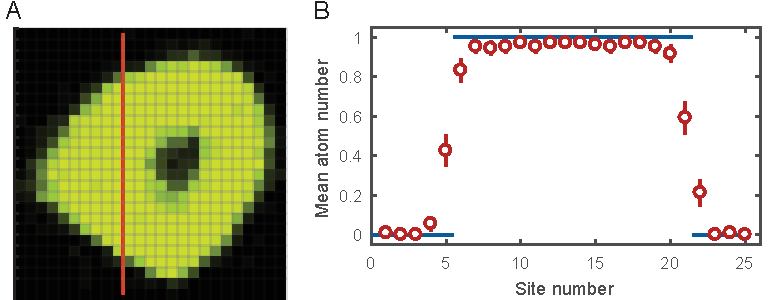
\includegraphics[scale=1]{figures/CTE_MI.pdf}
	\caption{{\bf Encoding phase and amplitude information with a grating}. {\bf A} When a light with initial wave vector $K_0$ passes through an amplitude grating with period $d$, it's outgoing wave vector can be changed by any integer multiple of grating wave vector $K_g\propto \frac{1}{d}$. {\bf B} Tow patches with the grating of the same period $d$ but different duty cycles $q_1$ and $q_2$ are shown. Since the duty cycle determines how much light goes through, the intensity of the outgoing light is proportional to the duty cycle. The outgoing light also carries the information about the local phase of the grating, by imprinting it onto the phase of the outgoing electric field.}
	\label{fig:CTE_MI}
\end{figure*}

An alternative route is a top-down approach, where one uses an ensemble of atoms to, first, create a macroscopic number of atoms in the absolute ground state \cite{BEC, DFG}, then selectively remove all exited state atoms \cite{ammy's thesis}, and finally adiabatically load them into an optical lattice \cite{Greiner2002}. By ramping up the lattice depth the ratio between interaction and kinetic energies of the atoms can be increased. And at the critical ratio between those energy scales the system enters a Mott insulating phase (see fig.~\ref{fig:CTE_MI}A), where each lattice site is occupied by an integer number of atoms according to a local chemical potential, with a vanishing atom number variance \cite{Bakr2010, Bloch MI}. However, since at the phase transition the gap between the ground and the exited state closes, it is impossible to cross the transition completely adiabatically in a finite amount of time \cite{subir phase transition}. Therefore at the end of the ramp the system has a small admixture of low lying exited states, resulting in  deviations of the atom number distribution from the ground state one by "smearing" the boundary between the shells with different occupation numbers (see fig~\ref{CTE_MI}B). However, if the Mott insulator is sufficiently large, we can find a region with nearly unity filling up to $12$ sites long. Hence, to achieve our desired target state, we just need to isolate such a region and ensure that it doesn't get disturbed by the adjacent atoms during subsequent evolution.

\section{Cutting procedure}

In order to isolate a desired region of the lattice, we perform a so-called "cutting" procedure. Using the DMD we project a finite size lattice potential on top of the initial $2\mathrm{D}$ lattice, in which the Mott insulator was originally created. Then, by applying a slowly varying repulsive beam and switching off the $2\mathrm{D}$ lattice, we make the atoms leave, except for those that were kept by the DMD potential (see fig.~\ref{fig:CTE_cutting}B). Finally, we can reload the atoms into the $2\mathrm{D}$ lattice by ramping it back up and switching off the DMD potential. By repeating this procedure along both directions, we isolate plaquettes up to $12\times2$ in size (see fig.~\ref{fig:CTE_cutting}C). This technique allows us to achieve $99\%$ single atom transfer fidelity from the initial Mott insulator. The preparation of larger systems could be achieved by increasing the optical power of the DMD beam. Similar results have been achieved using state-dependent light shifts and microwave pulses \cite{Bloch single site addresing}.

\begin{figure*}[t]
	\centering
	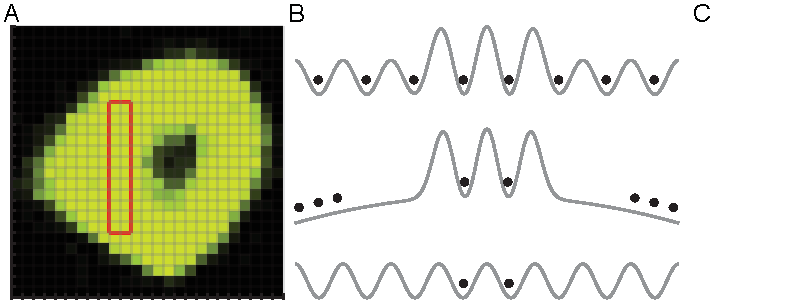
\includegraphics[scale=1]{figures/CTE_cutting.pdf}
	\caption{{\bf Encoding phase and amplitude information with a grating}. {\bf A} When a light with initial wave vector $K_0$ passes through an amplitude grating with period $d$, it's outgoing wave vector can be changed by any integer multiple of grating wave vector $K_g\propto \frac{1}{d}$. {\bf B} Tow patches with the grating of the same period $d$ but different duty cycles $q_1$ and $q_2$ are shown. Since the duty cycle determines how much light goes through, the intensity of the outgoing light is proportional to the duty cycle. The outgoing light also carries the information about the local phase of the grating, by imprinting it onto the phase of the outgoing electric field.}
	\label{fig:CTE_cutting}
\end{figure*}

By increasing the DMD beam power we could in principal initialize even longer chains, however, there is another difficulty in our system. In order to achieve a high fidelity of the $n=1$ shell of the Mott insulator, we rely on the idea of entropy redistribution in the system \cite{some entropy redistribution}. This concept can be applied to our system in the following way: crossing the transition from a Superfluid to a Mott insulator at finite time injects a certain amount of particle-hole excitations into the system. If the system would be homogeneous those excitations would spread evenly across the system. However, there is a strong inhomogeneity in the regions where shells of different occupation number touch one another. Since the density has to smoothly connect from one occupation to another, it deviates from an integer value creating regions of superfluid. A superfluid has a significantly smaller gap between low lying states compared to a Mott shell, hence it is energetically favourable for the excitations to concentrate in the regions between the shells. From the above considerations, it is clear that this mechanism works better for a larger ratio of the superfluid region to the Mott shells. An analogous technique has also found a great success in Fermi gas microscopes, where a manual increase of the entropy reservoir region led to significant entropy reductions in the gapped part of the system \cite{Mazurenko2017, Chiu2018}.

\begin{figure*}[t]
	\centering
	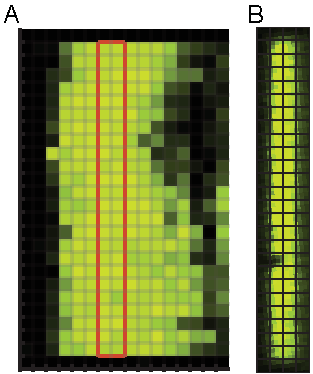
\includegraphics[scale=1]{figures/CTE_MI_box.pdf}
	\caption{{\bf Encoding phase and amplitude information with a grating}. {\bf A} When a light with initial wave vector $K_0$ passes through an amplitude grating with period $d$, it's outgoing wave vector can be changed by any integer multiple of grating wave vector $K_g\propto \frac{1}{d}$. {\bf B} Tow patches with the grating of the same period $d$ but different duty cycles $q_1$ and $q_2$ are shown. Since the duty cycle determines how much light goes through, the intensity of the outgoing light is proportional to the duty cycle. The outgoing light also carries the information about the local phase of the grating, by imprinting it onto the phase of the outgoing electric field.}
	\label{fig:CTE_MI_box}
\end{figure*}

From the analysis above it follows, that in order to create $n=1$ shell with high fidelity, it is advantageous to have it surrounded by $n=0$ and $n=2$ shells. The current trapping geometry allows us to create chains of up to $\sim 16$ sites long. For even longer chains their single site fidelities become effected by the residual disorder of the lattice potential. One way to overcome this issue is to alter our trapping geometry. One simple solution that comes to mind is to make a rectangular box confinement instead of a harmonic one. In order to have well-defined shells, in this case, one can use a magnetic field gradient in order to create a uniform tilt. We realize such a configuration in our system in a $24$ site long box (see fig.~\ref{fig:CTE_MI_box}), then by using a cutting procedure along the other direction we were able to achieve $24\times 2$ plaquettes. In this case, the length was only limited by the DMD beam power, that provided the confinement during the cutting procedure. By increasing the DMD power and reducing the disorder, coming from $2D$ lattice, this approach can enable the initialization of even longer chains of controlled length, which are particularly interesting for quantum simulations.

\section{Atoms life time}
In our experiments we are interested in studying coherent quantum many-body dynamics on sufficiently long timescales. In order to achieve that, we need to isolate our system from coupling to the environment. Working with neutral atoms gets up a very good head start, since they can only interact with the environment is through collisions with photons or background atoms. Let's look at the later process in more detail.

\begin{figure*}[t]
	\centering
	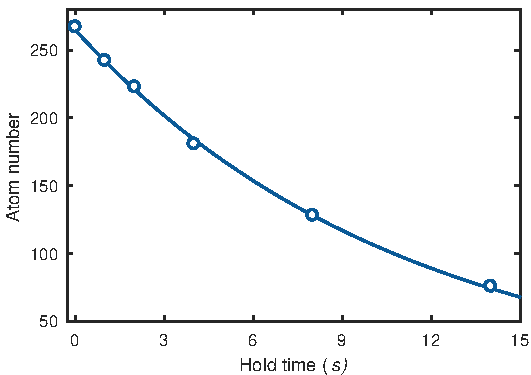
\includegraphics[scale=1]{figures/CTE_lifetime.pdf}
	\caption{{\bf Encoding phase and amplitude information with a grating}. {\bf A} When a light with initial wave vector $K_0$ passes through an amplitude grating with period $d$, it's outgoing wave vector can be changed by any integer multiple of grating wave vector $K_g\propto \frac{1}{d}$. {\bf B} Tow patches with the grating of the same period $d$ but different duty cycles $q_1$ and $q_2$ are shown. Since the duty cycle determines how much light goes through, the intensity of the outgoing light is proportional to the duty cycle. The outgoing light also carries the information about the local phase of the grating, by imprinting it onto the phase of the outgoing electric field.}
	\label{fig:CTE_liefetime}
\end{figure*}

In order to understand the effect of collisions with background gas one needs to consider the energy scales in the system. The typical depth of the optical potentials, that we use to confine our atoms, is on the order of $1 \mu \textrm{K}$. In contrast, since the vacuum chamber walls are at room temperature, the typical energy of the background gas is $300 \textrm{K}$. Hence, a collision between the atom within our system with a background gas atom will lead to the atom loss. This means, that by measuring the atom loss rate in our system, we can determine the timescale corresponding to this process. To measure it, we prepare atoms in a shallow harmonic optical trap and image them after variable amount of holding time (see fig.~\ref{fig:CTE_lifetime}). We measure a single particle $\frac{1}{e}$ decay time of of $21.4(7)\textrm{s}$ in our system. For a $10$ particles  evolving for $1\textrm{s}$ this results in $\sim 40\%$ probability of single particle loss, that would lead to decoherence in the system.

However, if we work with the systems of fixed particle number, the above source of decoherence can be overcome in our experiments. The high fidelity initial state preparation allows us to start with a known number of atoms at the beginning of the experiment. If we could also determine the total number of atoms at the end of the sequence, we could discard the experimental runs in which the total atom number in the beginning and at the end are different. This procedure would eliminate the decoherence due to the atom loss at the expanse of the number of successful runs of the experiment.

\section{Atom number resolved state readout}
One of the drawbacks of quantum gas microscopes is so-called parity projection during the imaging process. When subject to resonant light two atoms undergo photon assisted collisions, resulting in the formation of a molecule with a large kinetic energy. The molecules are not trapped by the optical lattice and get lost during this process. This means, that in our image the sites with two particles on the same site appear dark like an empty site and the sites with three particles appear as one. Although it is not a problem in the Mott insulator regime, it leads to the loss of large amounts of information about the state in the superfluid regime. 

We can utilize the direction transverse to the chain, in order to achieve full number resolution for a one-dimensional system. The idea behind this method is simple: once the dynamics along the chain is frozen (in our case we do this by rapidly increasing the lattice depth along the chain to $45 \mathrm{E_{r}}$), we can switch the confinement transverse to the chain (which is provided by the other optical lattice in this case) to spread the atoms from every site of the chain into tubes $\sim 80$ lattice sites long in the transverse direction. In this case, the probability of doubly occupying any site of the tube is given by
\begin{equation}
p(n,L) = \sum_{i=1}^{n-1}\frac{i}{L},
\end{equation}
where $n$ is the number of particles that start on the site in the beginning and $L$ is the length of the expansion tube in lattice sites. An example of such a process is shown in figure \ref{fig:CTE_fullcounting}.

\begin{figure*}[t]
	\centering
	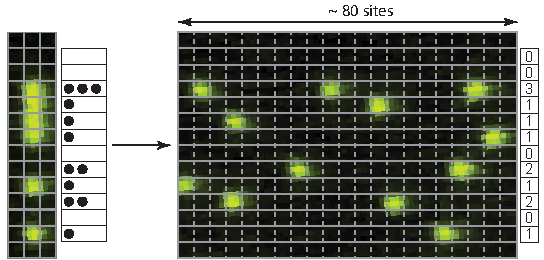
\includegraphics[scale=1]{figures/CTE_fullcounting.pdf}
	\caption{{\bf Encoding phase and amplitude information with a grating}. {\bf A} When a light with initial wave vector $K_0$ passes through an amplitude grating with period $d$, it's outgoing wave vector can be changed by any integer multiple of grating wave vector $K_g\propto \frac{1}{d}$. {\bf B} Tow patches with the grating of the same period $d$ but different duty cycles $q_1$ and $q_2$ are shown. Since the duty cycle determines how much light goes through, the intensity of the outgoing light is proportional to the duty cycle. The outgoing light also carries the information about the local phase of the grating, by imprinting it onto the phase of the outgoing electric field.}
	\label{fig:CTE_fullcounting}
\end{figure*}

Although this technique is very powerful for isolated one dimensional systems, we would like to develop a method that would allow us to perform counting of a $2\times N$ plaquettes. At first, the solution seems very simple: one just needs a way to isolate the two sides of the plaquette and repeat the above procedure. Using the DMD we can project a single site-wide Gaussian beam to disable the tunnelling between the two sides of the plaquette. However, that leads to an issue: the potential, required to completely suppress the hopping between the two sides, has a sufficient height at the position of the atoms, serving as an effective hill the atoms roll down from. This process imparts a momentum onto the atoms in the direction away from the barrier potential, which is large compared to the diffusion rate of the atoms. The result is that the atoms can only spread across $\sim 20$ lattice sites before they leave the field of view of the microscope (see fig.~\ref{fig:CTE_expansion}~A). Such limited spread results in a significant probability of double occupancies.

\begin{figure*}[t]
	\centering
	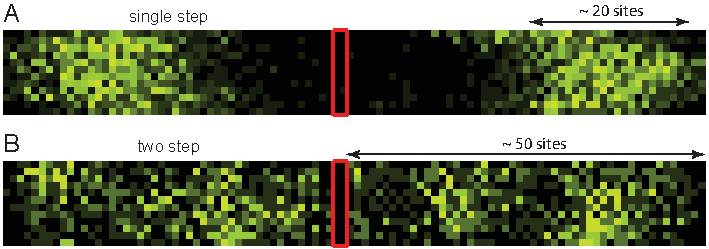
\includegraphics[scale=1]{figures/CTE_expansion.pdf}
	\caption{{\bf Encoding phase and amplitude information with a grating}. {\bf A} When a light with initial wave vector $K_0$ passes through an amplitude grating with period $d$, it's outgoing wave vector can be changed by any integer multiple of grating wave vector $K_g\propto \frac{1}{d}$. {\bf B} Tow patches with the grating of the same period $d$ but different duty cycles $q_1$ and $q_2$ are shown. Since the duty cycle determines how much light goes through, the intensity of the outgoing light is proportional to the duty cycle. The outgoing light also carries the information about the local phase of the grating, by imprinting it onto the phase of the outgoing electric field.}
	\label{fig:CTE_expansion}
\end{figure*}

To overcome this issue we add another step to this process. After a very short expansion time, when the atom distribution has moved by a few sites away from the barrier, and its effect can be neglected. We briefly capture the atoms back into the lattice and then release them again. This process randomizes the momentum of each atom and allows them to expand into the corresponding half tube with zero centres of mass momentum. This allows us to spread the occupation of a single site of the plaquette into $\sim 50$ lattice sites, resulting in the $94\%$ probability of successfully detecting $3$ atoms or less. 